\documentclass[11pt,a4paper]{article}
\usepackage[latin1]{inputenc}
\usepackage{amsmath}
\usepackage{amsfonts}
\usepackage{amssymb}
\usepackage{makeidx}
\usepackage{graphicx, array}
\usepackage{pgf,tikz}
\usepackage{tkz-euclide}
\usetkzobj{all}
\pagestyle{empty}
\usepackage{pgfplots}
\pgfplotsset{compat=1.9}
\usepackage{enumerate}
\usepackage[margin = 0.5in]{geometry}
\raggedright



\begin{document}

Name \makebox[2.5in]{\hrulefill}    \hfill  \textbf{Properties of Functions}
\newline\\
Period \makebox[0.35in]{\hrulefill} \newline\\

\fbox{\emph{Level 1}}   \newline\\

Let $f(x)=\begin{cases}
x+5 \quad   \text{ if } &   x \leq -2   \\
\sqrt{9-x^2}    \quad   \text { if } & -2<x\leq 2   \\
-x+5    \quad   \text{ if } &   x>2 \\
\end{cases}$ \quad Compute the following function values.
\begin{flalign*}
1.  \quad   &   f(-3)       &
2.  \quad   &   f(-2)       &
3.  \quad   &   f(2)        &
4.  \quad   &   f(2.001)    &
5.  \quad   &   f(-2.001)   &
6.  \quad   &   f(0)        &&\\[0.5in]
\end{flalign*}

Determine if each of the following are even, odd, or neither.
\begin{flalign*}
7.  \quad   &   f(x)=3x^2-4         &
8.  \quad   &   f(x)=4-5x^2         &
9.  \quad   &   f(x)=x^2-2x-6       &&\\[1in]          
10. \quad   &   f(x)=2x^3-x         &
11. \quad   &   f(x)=-x^5+6x^3-7x   &
12. \quad   &   f(x)=x^6-x^4+x^2+7  &&\\[1in]
\end{flalign*}


Use the graph to answer the following about $g(x)$.
\newline\\

\begin{minipage}{0.5\linewidth}
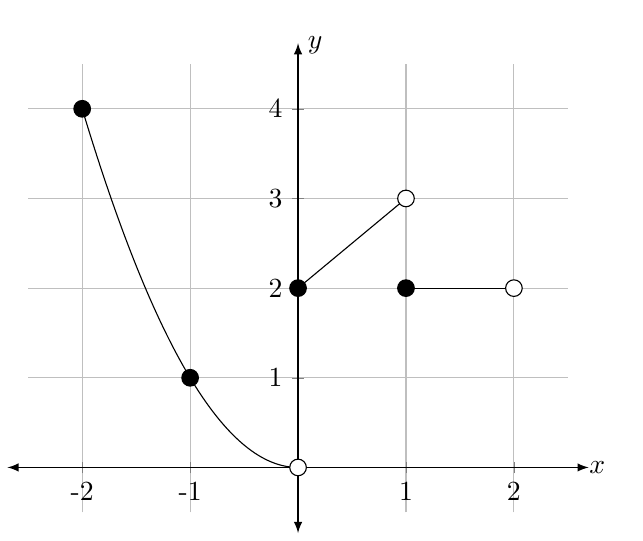
\begin{tikzpicture}

\begin{axis}
[   
    grid,
    axis lines=middle,
    xmin=-2.5,xmax=2.5,
    ymin=-0.5,ymax=4.5,
    restrict y to domain=-1:5,
    xtick={-2,-1,...,2},
    xticklabels={-2,-1,,1,2},
    ytick={0,1,...,4},
    yticklabels={,1,2,3,4},
    axis line style={latex-latex},
    axis line style={shorten >=-7.5pt, shorten <=-7.5pt},
    xlabel=$x$,
    ylabel=$y$,
    xlabel style={at={(ticklabel* cs:1)},anchor=west, xshift=0.15cm},
    ylabel style={at={(ticklabel* cs:1)},anchor=south west}
]

\addplot [domain = -2:0, samples = 500]{x*x};
\addplot [mark = *, mark size=3pt] coordinates {(-2,4)};
\addplot [mark = *, mark size=3pt] coordinates {(-1,1)};
\addplot [mark = *, mark size=3pt, fill=white] coordinates {(0,0)};
\addplot [domain = 0:1, samples = 500] {x+2};
\addplot [mark = *, mark size=3pt] coordinates {(0,2)};
\addplot [mark = *, mark size=3pt, fill=white] coordinates {(1,3)};
\addplot [domain = 1:2, samples = 500] {2};
\addplot [mark = *, mark size=3pt] coordinates {(1,2)};
\addplot [mark = *, mark size=3pt, fill=white] coordinates {(2,2)};

\end{axis}
\end{tikzpicture}
\end{minipage}
\hspace{-0.5in}
\begin{minipage}{0.4\linewidth}
13. Domain of $g$   \\[0.35in]
14. Range of $g$    \\[0.35in]
15. $g(1)$          \\[0.35in]
16. Solve $g(x)=1$  \\[0.35in]
17. Where is $g(x)$ increasing? \\[0.35in]
18. Where is $g(x)$ decreasing? \\[0.35in]
19. Where is $g(x)$ constant?   \\[0.35in]
20. List the maximum and minimum of $g(x)$.
\end{minipage}

\newpage

\fbox{\emph{Level 2}}   \newline\\

Describe the graph of a function $f$ that is continuous on the interval $[5, -5]$, except as noted. Sketch the graph of each function.
\newline\\

21. The function is increasing on $[-5, 0)$, discontinuous at $x=0$, increasing on $(0,5]$, $f(-2)=0$ and $f(2)=0$. \vspace{2in}

22. The function $f$ is discontinuous at $x=-2$ and $x=2$, $f(-3)=2$ and $f(3)=2$ are local minima, and $f(0)=0$ is a local maximum.    \vspace{2in}


\fbox{\emph{Level 3}}   \newline\\

Find the domain, range, and any points of discontinuity for each.
\begin{flalign*}
23. \quad   &   f(x)=\dfrac{|5x-10|}{x-2}   &
24. \quad   &   f(x)=x+\dfrac{|2x+2|}{x+1}  &
25. \quad   &   f(x)=|x|-\dfrac{|9-3x|}{x-3}&&\\
\end{flalign*}


\newpage


\textbf{Properties of Functions KEY}
\newline\\


\begin{enumerate}
    \item 2
    \item 3
    \item 2.236
    \item 2.999
    \item 2.999
    \item 3
    \item even
    \item even
    \item neither
    \item odd
    \item odd
    \item even
    \item $[-2, \, 2)$
    \item $(0, \, 4]$
    \item 2
    \item $x = -1$
    \item (0, 1)
    \item (--2, 0)
    \item (1, 2)
    \item max = (--2, 4), min = none
\end{enumerate}


\end{document}
